\documentclass[11pt,a4paper]{article}
\usepackage{alex-report}
\ReportSetup{DSpecM1D scientific validation}{Study 2}{3 November 2026}
\hypersetup{pdftitle={DSpecM1D study 2: finite convergence controls}}
\begin{document}
\ReportTitle{Finite convergence controls}{Radial resolution is stable; angular cutoff is not yet stabilized}
\textbf{Finding.} The observed radial-refinement and NQ changes are below 0.1\% for the waveform, measurement normalization and selected far-solid-interior kernel vector. The physical angular cutoff is a different limitation: L200 to L300 changes the whole velocity trace by 4.16\% and the selected far-interior kernel vector by 165.90\%. YSpec shows essentially the same degree dependence. Close agreement between codes at fixed L does not establish convergence to the continuum problem.

\section{Case, controls and meaning of the numbers}
This is the same attenuated anisotropic PREM transverse-velocity traveltime fixture as Study 1: source depth 29.5 km; solid-side receiver at the 3 km solid--fluid boundary; 60-degree separation; 1000--1200 s window with 40 s taper; existing 2/4/8/10 mHz filter. All 35 bins, full gravity and full radial systems are retained. The kernel parameter is $\ln V_s$ at fixed $V_p$, density and effective $Q$.

Eleven new sequential solver jobs were run on Tunya in isolated directories. DSpec used eight frequency workers and YSpec eight outer workers, each with one inner library thread. Physical degree cutoffs were L100, L150, L200 and L300. YSpec's radial ODE tolerance was fixed at $10^{-7}$. Each unperturbed case used its own waveform-derived adjoint weights. The L200 reference comes from the accepted first study.

All percentages below are $100\|b-a\|_2/\|a\|_2$ for the named discrete sample vectors, except the normalization column, which is $100|N_b/N_a-1|$. The far-interior vector contains 89 fixed probes in solid material, away from material interfaces and at least 100 km from both source and receiver; source-shell traces are excluded. These are sample-vector diagnostics, not three-dimensional $L^2$ or $H^1$ norms or universal pointwise error bounds.

\section{Radial resolution and polynomial/quadrature order}
\begin{center}\small\begin{tabular}{lrrr}\toprule
Change at L200 & Velocity (\%) & Far kernel (\%) & $|\Delta N|$ (\%)\\\midrule
$h_0\to0.75h_0$ & 0.000079 & 0.000163 & 0.000003 \\
$0.75h_0\to0.5625h_0$ & 0.000039 & 0.000190 & 0.000012 \\
NQ6 to NQ8 & 0.000151 & 0.007439 & 0.000022 \\
NQ8 to NQ10 & 0.000057 & 0.000086 & 0.000004 \\
\bottomrule\end{tabular}\end{center}
The normalized mesh-step parameter is $h_0=0.02035382429229197$, not a length in metres. The mesh has 59, 75 and 95 elements on the three $h$ levels; maximum physical element widths are 125.472, 94.104 and 72.855 km. NQ6, NQ8 and NQ10 use exactly the same 59-element boundaries at $h_0$. Thus increasing NQ is not confounded with a mesh change. NQ6 versus NQ10 changes the selected far-interior vector by 0.007464\%; NQ8 versus NQ10 is smaller still.

These controls support the current radial discretization for this finite-L fixture. They do not transfer the 0.1\% statement to an untested angular cutoff, every point or a singular-limit norm. YSpec's sampled radial mesh is an output grid; it is not an independent YSpec ODE refinement control.

\newpage
\section{Physical angular cutoff: unresolved convergence}
\begin{center}\small\begin{tabular}{lrrr}\toprule
Change & Velocity (\%) & Far kernel (\%) & $|\Delta N|$ (\%)\\\midrule
DSpec L100 to L150 & 2.298501 & 70.233670 & 1.024326 \\
DSpec L150 to L200 & 4.766502 & 161.709918 & 1.762785 \\
DSpec L200 to L300 & 4.162965 & 165.898562 & 1.439444 \\
YSpec L100 to L150 & 2.298500 & 70.233947 & 1.024326 \\
YSpec L150 to L200 & 4.766500 & 161.715516 & 1.762785 \\
YSpec L200 to L300 & 4.162963 & 165.889172 & 1.439443 \\
\bottomrule\end{tabular}\end{center}
\begin{figure}[H]\centering
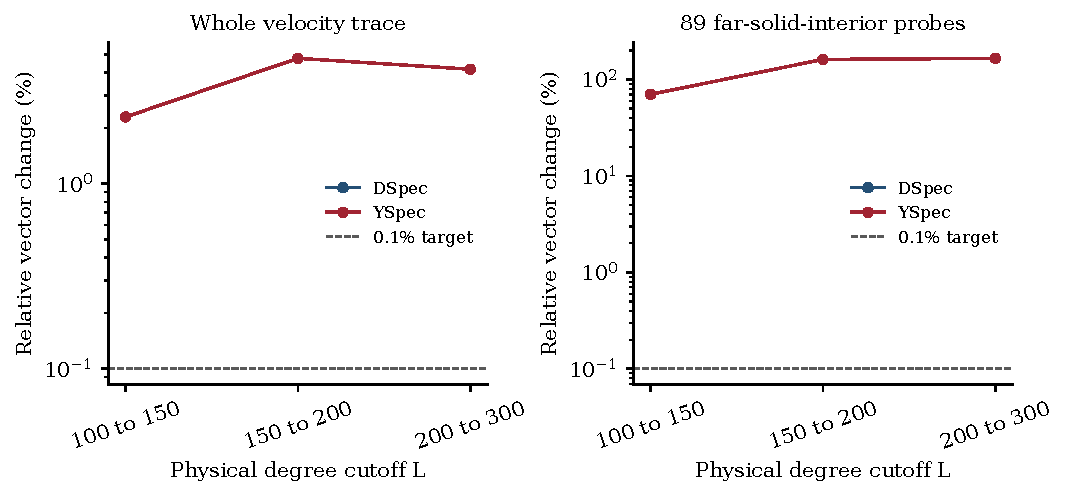
\includegraphics[width=\linewidth]{figures/study2-degree-controls.pdf}
\caption{Actual adjacent cutoff changes with each case's own waveform-derived adjoint weights. Curves for the two codes nearly overlap. The dashed line is a 0.1\% observed-change target, not an established error estimator. Fixed probes are reused; their vector norm has no volume weights.}
\end{figure}
The L200-to-L300 DSpec velocity change within the nonzero measurement-window samples alone is 0.872500\%, so the discrepancy is not confined to times outside the measurement. The measurement-rate normalization changes by $-1.43944$\%, and the adjoint-source vector changes by 0.794524\%. The selected far-interior kernel changes by 165.90\%, solid material-interface samples by 146.81\%, and source-shell inner/outer samples by 193.53\%. The latter remain contact-limited regular-volume samples.

The far-interior L200 vector norm is $8.71906\times10^{-15}$ and the L300 norm is $2.00077\times10^{-14}$; their difference norm is $1.44648\times10^{-14}$ in the sampled kernel units. This is a material change, not merely a percentage computed at one near-zero point. It does not prove divergence. The nonmonotone finite ladder does not establish an asymptotic rate or a sufficient final L. No L greater than 300 was run.

\newpage
\section{Agreement between the two implementations}
\begin{center}\small\begin{tabular}{lrrr}\toprule
Matched cutoff & Velocity (\%) & Far kernel (\%) & $|\Delta N|$ (\%)\\\midrule
L100 & 0.000116 & 0.000426 & 0.000026 \\
L150 & 0.000116 & 0.002388 & 0.000026 \\
L200 & 0.000116 & 0.007503 & 0.000025 \\
L300 & 0.000116 & 0.004584 & 0.000026 \\
\bottomrule\end{tabular}\end{center}
The denominator here is DSpec's vector norm, and both implementations use their own waveform-derived weights. These small discrepancies establish agreement for the matched finite-cutoff calculations on the supported sample cohort. They do not establish that the common finite-cutoff answer is accurate to 0.1\% against a converged angular solution.

Source-shell traces unavailable through YSpec's public interface are not included in the matched far-interior comparison. The Study 1 source-radius trace mismatch remains a separate interpretation issue. The receiver functional is unchanged on the solid side of the physical solid--fluid interface. No smoothing, new $H^1$ gradient, source regularization, receiver averaging or singular-contact correction was implemented.

\section{Finite samples and the source/receiver question}
All saved native section samples are finite. This cannot establish bounded continuum values near ideal point sources or receivers. Neither this study nor Study 1 proves or disproves a singular limit, global $H^1$ regularity or a valid pointwise product at contact. The source-shell regular-volume samples and any omitted distributional contact contributions must not be interchanged.

The output sections deliberately use a common sparse grid of 68 along-path and 10 cross-path angles while the actual solved degree changes up to L300. Sparse section extrema remain unmasked in the saved evidence, but they are sampled extrema, not global angular maxima. The 168 fixed probes provide exact matched physical positions for the control comparisons. The historical vertical-displacement energy example was not rerun and is not certified by this traveltime study.

\section{Validation record and stopping point}
All 11 jobs completed cleanly, with unchanged declared inputs and verified cleanup. The root retrieval rehashed 197 outputs/logs plus the exact finalized state. The standalone checker passed after one reviewed provenance-only correction: the absolute model path in \texttt{parameters.txt} necessarily differs between the isolated Study 1 and Study 2 folders. Both model hashes and every non-path byte were checked. The failed first checker state and log are retained; no numerical job was rerun.

The checker status PASS means that the planned finite controls and evidence checks passed. It does not mean the angular solution converged. Sol 6.1 independently recomputed the trends from raw outputs, in addition to its plan, source, build and terminal reviews. Resource peaks were 9 threads and approximately 1.82 GiB under the accepted user-space watchdog; these are not kernel aggregate accounting.

The supported conclusion is radial stability and close cross-code agreement at fixed L, with unresolved angular-cutoff convergence. Study 1's supported smooth-perturbation directional derivative check remains valid within its own low-degree scope. All changes and results remain isolated. Production integration, higher-cutoff work and further optimization have not been started.

\medskip\noindent\small Evidence: \texttt{study2-v1/evidence/producer-raw-v1/}; standalone checker report and independent raw metrics are retained alongside the editable report generator. Frozen producer state SHA-256 begins \texttt{9cd09f3e}; checker report begins \texttt{aedda47c}. The delivery manifest records full hashes.
\end{document}
